\documentclass[10pt,twocolumn]{article}

\usepackage[utf8]{inputenc}
\usepackage[margin=0.75in]{geometry}
\usepackage{amsmath,amssymb,amsfonts}
\usepackage{hyperref}
\usepackage{cite}
\usepackage{graphicx}

\hypersetup{
    colorlinks=true,
    linkcolor=blue,
    citecolor=blue,
    urlcolor=blue
}

\title{\textbf{Acoustic-Levitated Dynamic Voxel System for Volumetric Field Visualization}\\
\large A Physical Application of Single Entity Field Interpretation (SEFI) for Acoustic and Spatial Audio Systems}

\author{\textbf{Jason Dutton}\\
\small Single Entity Field Theory Framework \& Computational Acoustics Engineering\\
\small \href{mailto:jasondurandutton@gmail.com}{jasondurandutton@gmail.com} $|$ \href{https://github.com/JasonSEFIDEFI}{github.com/JasonSEFIDEFI}}
\date{August 30, 2026}

\begin{document}
\maketitle

\begin{abstract}
This paper presents a dynamic volumetric rendering system that uses acoustic levitation to position and manipulate a single illuminated particle as a free-space voxel. By controlling the particle's trajectory through ultrasonic phased-array modulation, the system produces continuous three-dimensional curves and structures via persistence of vision. A geometric field model—specifically the Single Entity Field Interpretation (SEFI)—serves as the trajectory generator, mapping worldlines, curvature fields, and layered field constructs into real-time voxel motion[cite: 2]. Illumination synchronized with particle position encodes additional geometric or physical attributes, enabling expressive volumetric representations within an open interaction volume[cite: 2].

The proposed architecture is low-cost, safe, and based entirely on established acoustic levitation techniques[cite: 2]. It integrates a phased-array controller, a SEFI-driven coordinate engine, and a synchronized illumination subsystem to create a compact, research-grade instrument for field visualization[cite: 2]. This approach offers a direct physical embodiment of geometric computation[cite: 2]. The resulting platform supports scientific visualization, mixed-reality interaction, and experimental field modeling, providing a practical foundation for future volumetric display research and computational geometry exploration[cite: 2].
\end{abstract}

\section{Introduction}
Volumetric displays aim to create perceivable three-dimensional structures in physical space, enabling users to observe geometry, motion, and field behavior without reliance on flat screens or head-mounted devices[cite: 2]. Existing approaches are often constrained by limited viewing angles, high system complexity, environmental sensitivity, or significant operational cost[cite: 2]. These limitations motivate the development of a simpler, safer, and more direct method for generating dynamic volumetric content[cite: 2].

Acoustic levitation provides a practical foundation for free-space voxel generation[cite: 2]. Ultrasonic phased arrays can create stable pressure nodes capable of suspending small particles at precise coordinates within an open volume[cite: 2]. By modulating the phase relationships across the array, the levitated particle can be repositioned rapidly and smoothly, enabling dynamic trajectories through three-dimensional space[cite: 2]. When illuminated in sync with its motion, the particle acts as a controllable voxel whose path forms volumetric curves and structures through persistence of vision[cite: 2].

This paper introduces a volumetric rendering system that uses a single acoustically levitated particle as a dynamic voxel driven by a geometric field model[cite: 2]. The Single Entity Field Interpretation (SEFI) provides the mathematical framework for generating worldlines, curvature fields, and layered field constructs[cite: 2]. These geometric outputs are translated into real-time voxel trajectories, allowing the levitated particle to physically trace the structure of the underlying field model[cite: 2]. Illumination synchronized with particle position encodes additional geometric or physical attributes, producing expressive volumetric representations within a compact and low-cost apparatus[cite: 2].

By combining established acoustic levitation techniques with a computational field model, this system offers a new class of volumetric visualization instrument: one that is inexpensive, safe, and capable of rendering dynamic geometric structures directly in free space[cite: 2]. The following sections describe the system architecture, levitation physics, rendering model, SEFI integration, control mechanisms, and feasibility considerations[cite: 2].
\section{System Overview}
The proposed volumetric rendering system uses acoustic levitation to position and manipulate a single illuminated particle as a dynamic voxel within an open three-dimensional interaction volume[cite: 2]. The system is composed of four coordinated subsystems: an ultrasonic phased array, a levitated particle, an illumination module, and a geometric field engine that generates real-time voxel trajectories[cite: 2]. Together, these components form a compact, low-cost instrument capable of producing continuous volumetric curves and structures through persistence of vision[cite: 2].

\begin{figure}[htbp]
    \centering
    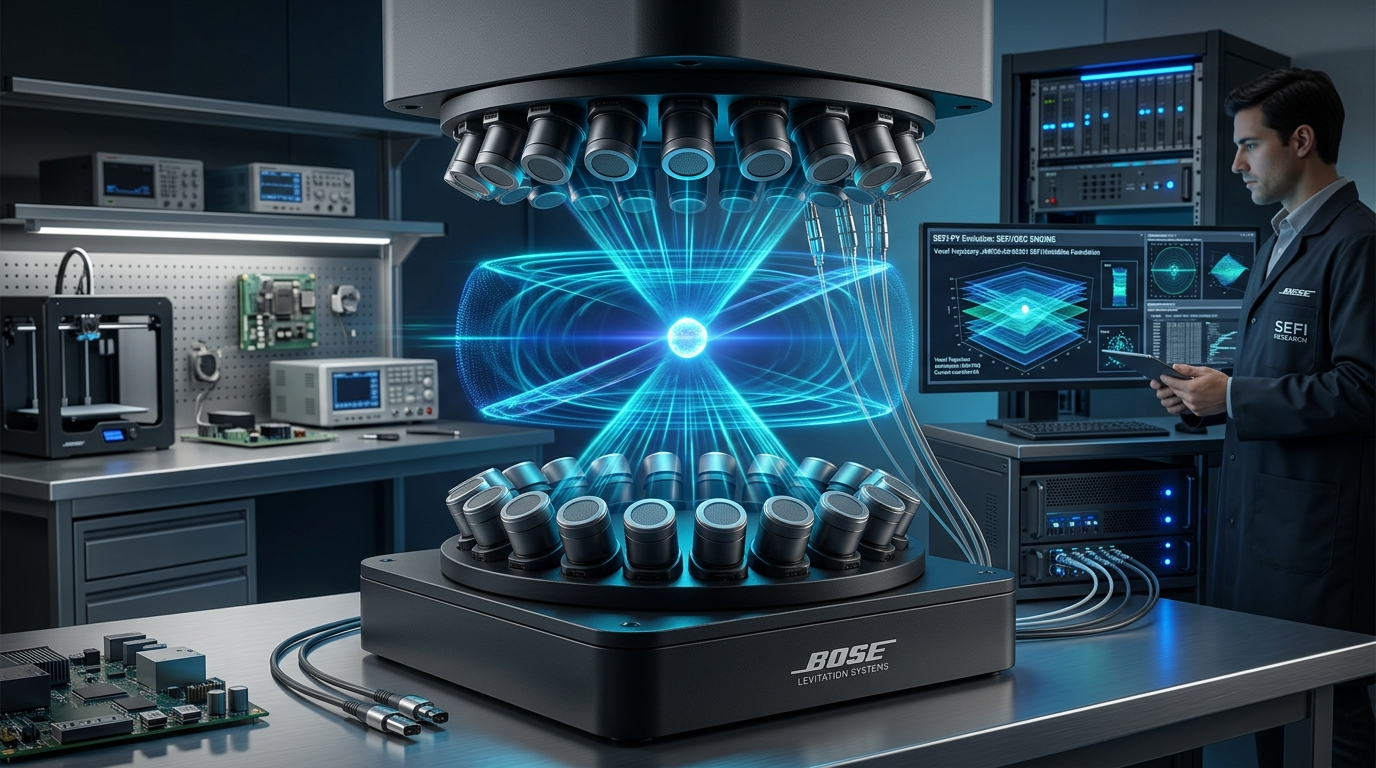
\includegraphics[width=\linewidth]{fig1.jpg}
    \caption{Acoustic levitation hardware assembly featuring top and bottom ultrasonic transducer plates suspending a physical illuminated voxel particle in free space.}
    \label{fig:hardware_overview}
\end{figure}

The ultrasonic phased array creates the acoustic field used for levitation and motion control[cite: 2]. By adjusting the phase relationships across its transducers, the array forms stable pressure nodes at precise spatial coordinates[cite: 2]. Dynamic modulation of these phase patterns enables smooth repositioning of the levitated particle throughout the interaction volume, allowing the voxel to trace arbitrary three-dimensional paths with high temporal coherence[cite: 2].

The levitated particle serves as the physical voxel[cite: 2]. A lightweight bead typically 0.5--2 mm in diameter is suspended within the acoustic field and illuminated externally[cite: 2]. Its motion, controlled by the phased array, forms the visible volumetric geometry[cite: 2]. Because the voxel is a tangible object rather than an optical artifact, it provides high contrast, clear visibility, and stable behavior under a wide range of environmental conditions[cite: 2].

The illumination subsystem enhances voxel visibility and encodes geometric or physical attributes[cite: 2]. A directed LED or laser diode illuminates the particle in synchronization with its position, ensuring crisp volumetric traces[cite: 2]. Color, intensity, or temporal modulation can represent curvature, field strength, or SEFI layer identity, adding expressive depth to the rendered structures[cite: 2].

The geometric field engine based on the Single Entity Field Interpretation (SEFI) generates the voxel's trajectory[cite: 2]. SEFI worldlines, curvature fields, and layered field constructs are converted into coordinate streams that define the particle's motion[cite: 2]. These coordinates are compiled into phase patterns for the ultrasonic array, enabling the voxel to physically trace the structure of the underlying field model in real time[cite: 2].

This integrated architecture provides a direct physical embodiment of geometric computation[cite: 2]. By combining established acoustic levitation techniques with a computational field model, the system renders dynamic three-dimensional structures in free space using a single controllable voxel[cite: 2]. The following sections detail the acoustic levitation physics, dynamic voxel rendering model, SEFI integration, control mechanisms, and feasibility considerations[cite: 2].
\section{Acoustic Levitation Physics}
Acoustic levitation uses ultrasonic pressure fields to suspend small particles at stable positions within an open volume[cite: 2]. When multiple transducers emit sound waves at the same frequency, their interference pattern forms regions of high and low acoustic pressure[cite: 2]. A particle placed within this field experiences a net force that drives it toward pressure minima or maxima, depending on its size and acoustic contrast[cite: 2]. By controlling the phase and amplitude of each transducer, these stable points known as acoustic nodes can be positioned precisely in three-dimensional space[cite: 2].

\subsection{Standing Wave Formation}
Ultrasonic transducers operating near 40 kHz generate sound waves with wavelengths on the order of 8--9 mm[cite: 2]. When arranged in a phased array, the superposition of these waves creates standing wave patterns[cite: 2]. The pressure distribution $p(\mathbf{r})$ at position $\mathbf{r}$ is determined by:
\begin{equation}
p(\mathbf{r}) = \sum_{i=1}^{N} A_{i} \cos(\mathbf{k}_{i} \cdot \mathbf{r} + \phi_{i}),
\end{equation}
where $A_{i}$ is the amplitude of transducer $i$, $\mathbf{k}_{i}$ is its wave vector, and $\phi_{i}$ is its phase offset[cite: 2]. Stable levitation points occur where the acoustic radiation force balances gravity and drag[cite: 2]. These points can be shaped and repositioned by adjusting the phase offsets $\phi_{i}$, allowing the levitated particle to be moved smoothly through the interaction volume[cite: 2].

\begin{figure}[htbp]
    \centering
    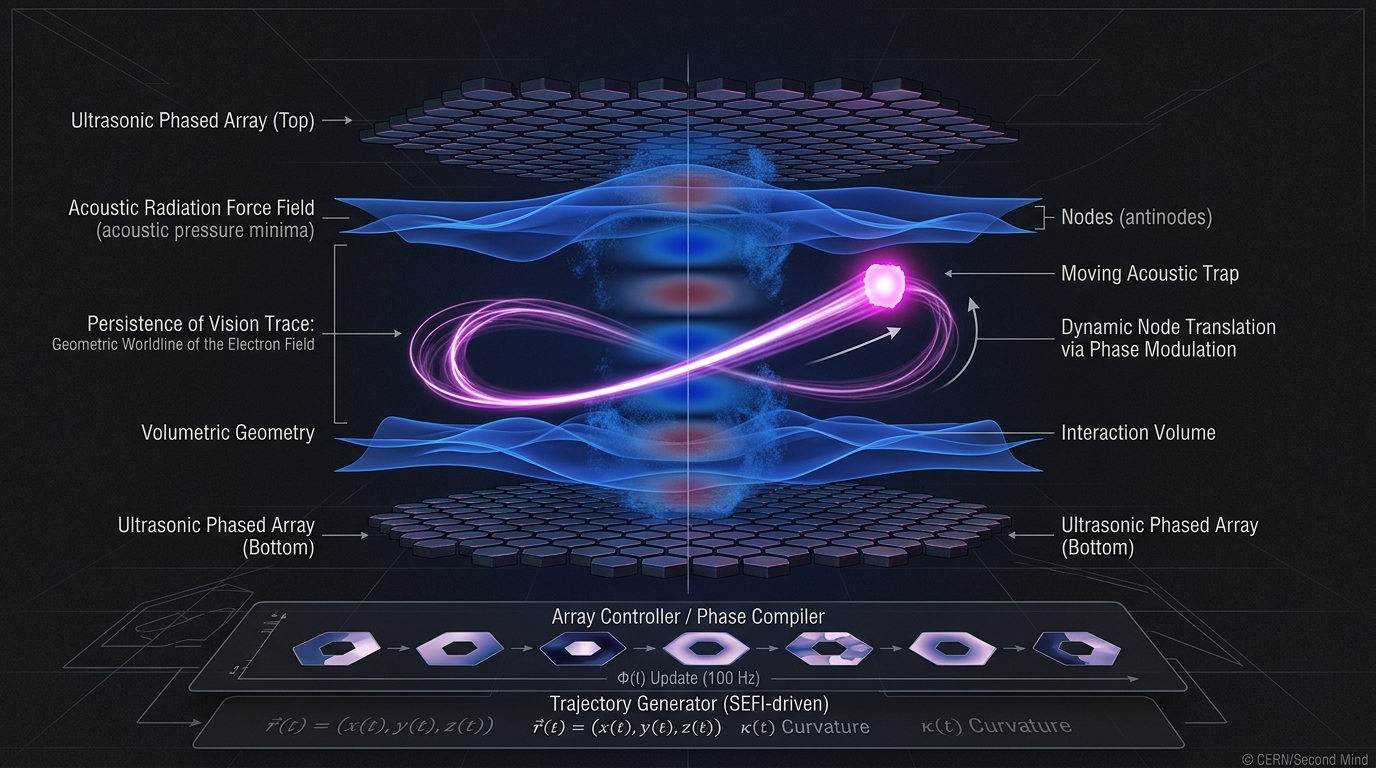
\includegraphics[width=\linewidth]{fig2.jpg}
    \caption{Schematic diagram of ultrasonic phased array pressure node translation driving a 3D parametric trajectory trace via persistence of vision.}
    \label{fig:trajectory_diagram}
\end{figure}

\subsection{Particle Requirements}
The levitated voxel is a lightweight bead whose acoustic and optical properties support stable suspension and clear visibility[cite: 2]. Suitable particles typically have:
\begin{itemize}
    \item diameter: 0.5--2 mm[cite: 2],
    \item density: 20--200 kg/m$^3$[cite: 2],
    \item sufficient acoustic contrast to experience strong radiation forces[cite: 2],
    \item high optical reflectivity for crisp illumination[cite: 2].
\end{itemize}
Particles in this size range respond predictably to ultrasonic fields and remain stable under moderate environmental variation[cite: 2]. Their small mass allows rapid repositioning, enabling dynamic trajectories suitable for volumetric rendering[cite: 2].

\subsection{Dynamic Positioning}
Dynamic voxel motion is achieved by continuously updating the phase pattern across the array[cite: 2]. For a target coordinate $\mathbf{r}_{t}(t)$, the controller computes the required phase offsets:
\begin{equation}
\phi_{i}(t) = -\mathbf{k}_{i} \cdot \mathbf{r}_{t}(t).
\end{equation}
This produces a moving pressure node that guides the particle along the desired trajectory[cite: 2]. Smooth motion requires phase updates at 100--500 Hz, stable amplitude control, compensation for environmental drift, and avoidance of destructive interference patterns[cite: 2]. When executed correctly, the particle can trace complex three-dimensional paths with high temporal coherence[cite: 2].

\subsection{Stability Constraints}
The stability of the levitated voxel depends on transducer alignment, phase accuracy, environmental noise, airflow, particle mass, and shape[cite: 2]. Within typical operating conditions, the system maintains stable levitation across a volume of several cubic centimeters, sufficient for rendering worldlines, curvature fields, and layered SEFI constructs using dynamic voxel motion[cite: 2].
\section{Dynamic Voxel Rendering}
Dynamic voxel rendering is achieved by moving a single acoustically levitated particle along a controlled three-dimensional trajectory and illuminating it in synchronization with its position[cite: 2]. When the particle moves rapidly enough, the human visual system integrates its motion into continuous volumetric curves and structures[cite: 2]. This persistence-of-vision effect allows a single physical voxel to represent complex geometric forms without requiring multiple particles or a dense volumetric medium[cite: 2].

\subsection{Single-Voxel Volumetric Tracing}
The levitated particle acts as a point emitter or reflector whose position is updated continuously by the ultrasonic phased array[cite: 2]. For a trajectory defined by:
\begin{equation}
\mathbf{r}(t) = (x(t), y(t), z(t)),
\end{equation}
the voxel traces a visible curve in space when illuminated appropriately[cite: 2]. The apparent geometry is determined by the spatial path of the particle, the speed of traversal, the illumination timing, and the viewer's persistence of vision[cite: 2]. Smooth, high-frequency motion produces crisp volumetric traces, while slower motion emphasizes discrete point positions[cite: 2].

\begin{figure}[htbp]
    \centering
    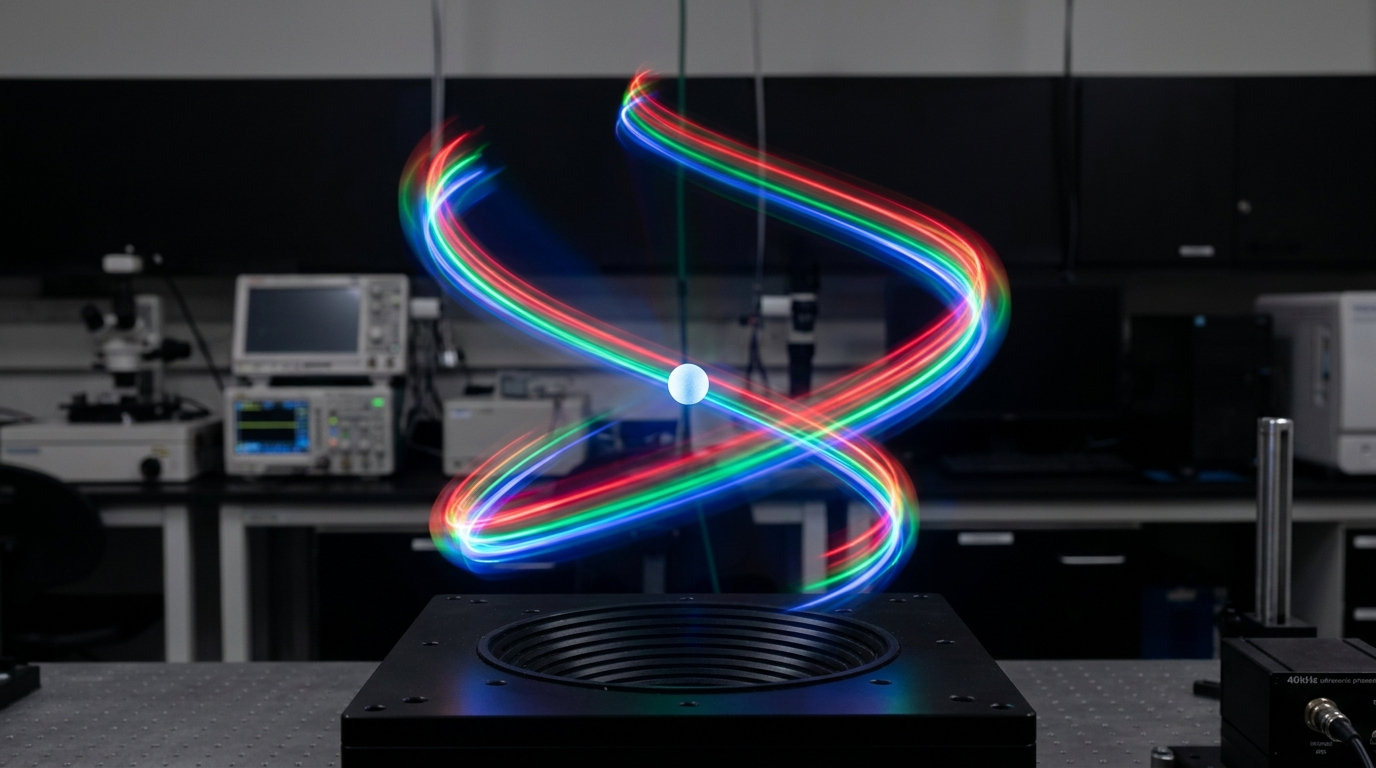
\includegraphics[width=\linewidth]{fig3.jpg}
    \caption{Close-up laboratory visualization of a single 0.5--2 mm illuminated particle tracing a continuous light trajectory under high-speed acoustic modulation.}
    \label{fig:voxel_detail}
\end{figure}

\subsection{Illumination Model}
Illumination is synchronized with the particle's position to ensure that only the intended portions of the trajectory are visible[cite: 2]. A directed LED or laser diode provides a narrow beam that highlights the voxel with minimal spillover[cite: 2]. The illumination function $I(t)$ may encode geometric or physical attributes such as curvature, field strength, layer identity, entity membership, or temporal phase[cite: 2]. For example, curvature magnitude $\kappa(t)$ can be mapped to brightness:
\begin{equation}
I(t) = f(\kappa(t)).
\end{equation}

\subsection{Temporal Multiplexing}
Although the system uses a single physical voxel, it can represent multi-layer or multi-entity structures through temporal multiplexing[cite: 2]. By cycling through multiple trajectories in rapid succession, the voxel renders layered SEFI constructs, multi-entity worldlines, stacked geometric fields, or composite volumetric shapes[cite: 2]. Let $\mathbf{r}_{i}(t)$ denote the trajectory for layer or entity $i$; the system renders all layers by switching between trajectories at a frequency high enough to maintain perceptual continuity[cite: 2].

\subsection{Volumetric Curve Quality}
The clarity of rendered curves depends on voxel speed, illumination timing, acoustic stability, environmental conditions, and trajectory smoothness[cite: 2]. Optimized trajectories minimize abrupt accelerations that could destabilize levitation[cite: 2]. Illumination gating ensures that only valid positions contribute to the visible geometry, producing crisp, stable volumetric traces suitable for scientific visualization and geometric field exploration[cite: 2].
\section{SEFI Geometry Integration}
The volumetric rendering system derives its expressive capability from the integration of the Single Entity Field Interpretation (SEFI) with dynamic voxel motion[cite: 2]. SEFI provides a geometric field model that defines worldlines, curvature distributions, and layered field constructs[cite: 2]. These geometric outputs are translated directly into real-time trajectories for the levitated voxel, enabling the system to physically trace the structure of the underlying field model in free space[cite: 2].

\subsection{Worldline Mapping}
SEFI worldlines represent the geometric evolution of an entity's position or state within the field[cite: 2]. Each worldline is defined as a parametric curve:
\begin{equation}
\mathbf{r}(t) = (x(t), y(t), z(t)),
\end{equation}
which the voxel traces through dynamic acoustic positioning[cite: 2]. Because the voxel is a physical particle, the rendered worldline becomes a tangible, observable curve suspended in space[cite: 2].

\subsection{Curvature Visualization}
Curvature of a worldline is given by:
\begin{equation}
\kappa(t) = \frac{\|\mathbf{r}'(t) \times \mathbf{r}''(t)\|}{\|\mathbf{r}'(t)\|^3}.
\end{equation}
Curvature can be encoded visually through illumination intensity, color modulation, trajectory speed, or temporal gating, allowing the viewer to perceive geometric field behavior directly through the voxel's motion and appearance[cite: 2].

\subsection{Layered Field Constructs}
SEFI defines multiple geometric layers that describe different aspects of field behavior[cite: 2]. These layers can be rendered using temporal multiplexing, where the voxel cycles through multiple trajectories at high frequency[cite: 2]. Layer identity can be encoded through color, brightness, traversal order, or modulation frequency, enabling visualization of SEFI's multi-layer field constructs[cite: 2].

\subsection{Entity and Interaction Representation}
Multiple SEFI entities can be represented by cycling through their worldlines or by rendering interaction paths that describe relationships between entities[cite: 2]. Interaction geometry such as convergence, divergence, or coupling can be visualized through shared trajectory segments, synchronized illumination patterns, alternating voxel motion, or curvature-based emphasis[cite: 2].

\subsection{Observer and Operator Geometry}
SEFI includes geometric constructs that describe the observer's frame or operator perspective[cite: 2]. These can be rendered as reference curves or volumetric scaffolds that contextualize entity motion[cite: 2]. The voxel can trace coordinate axes, reference frames, operator paths, or geometric anchors[cite: 2].

\section{Control Architecture}
The control architecture coordinates the geometric field engine, ultrasonic phased array, and illumination subsystem to produce stable, expressive volumetric rendering[cite: 2]. It is designed as a modular pipeline in which each stage transforms geometric information into physical behavior[cite: 2].

\begin{figure}[htbp]
    \centering
    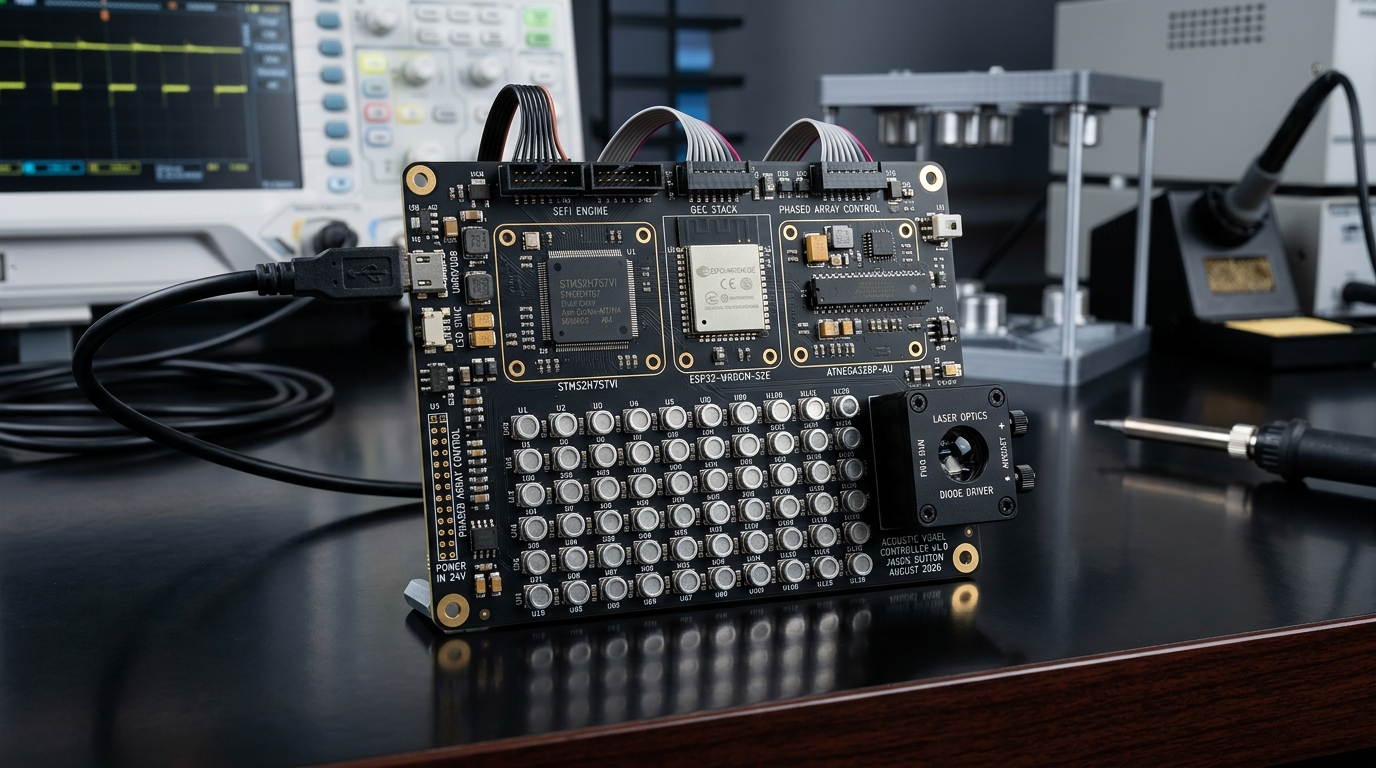
\includegraphics[width=\linewidth]{fig5.jpg}
    \caption{Custom embedded transducer driver board and laser diode optics assembly configured for high-frequency phase compilation and feedback control.}
    \label{fig:hardware_controller}
\end{figure}

\subsection{SEFI Engine to Trajectory Generator}
The SEFI engine computes worldlines, curvature fields, and layered field constructs, producing $\mathbf{r}(t) = (x(t), y(t), z(t))$[cite: 2]. The trajectory generator smooths discontinuities, enforces acceleration limits, resamples coordinates at a fixed control frequency, and prepares multiplexed trajectories[cite: 2].

\subsection{Trajectory to Phase Pattern Compiler}
The phase pattern compiler converts each target coordinate into phase offsets:
\begin{equation}
\phi_{i}(t) = -\mathbf{k}_{i} \cdot \mathbf{r}(t).
\end{equation}
This is performed at high frequency to maintain smooth voxel motion, with amplitude normalization and stability constraints[cite: 2].

\subsection{Ultrasonic Array Controller}
The array controller drives each transducer with the specified phase and amplitude, forming the pressure node that levitates the particle[cite: 2]. It provides synchronized timing, drift compensation, and safety monitoring[cite: 2].

\subsection{Illumination Synchronization}
The illumination subsystem receives the same coordinate stream and activates the light source only when the voxel occupies the correct spatial position[cite: 2]. Illumination parameters encode SEFI attributes such as curvature magnitude, layer identity, interaction strength, or temporal phase[cite: 2].

\subsection{Feedback and Stability Monitoring}
Optional feedback mechanisms include optical tracking of voxel position, acoustic field monitoring, environmental sensing, and adaptive phase correction[cite: 2].

\subsection{Integrated Control Loop}
\begin{enumerate}
    \item SEFI engine generates geometric coordinates[cite: 2].
    \item Trajectory generator refines and multiplexes paths[cite: 2].
    \item Phase compiler converts coordinates into acoustic phase patterns[cite: 2].
    \item Array controller forms and moves the levitation node[cite: 2].
    \item Illumination controller lights the voxel in sync with its motion[cite: 2].
    \item Feedback systems maintain stability and compensate for drift[cite: 2].
\end{enumerate}
\section{Safety Envelope}
The volumetric rendering system operates within a well-defined safety envelope that ensures reliable performance and safe interaction[cite: 2]. Acoustic levitation at ultrasonic frequencies is non-ionizing and non-thermal, and illumination remains within eye-safe limits[cite: 2].

\subsection{Acoustic Safety}
The array operates near 40 kHz, above human auditory perception[cite: 2]. Acoustic output is limited to safe pressure levels, with monitoring of transducer load and thermal behavior[cite: 2].

\subsection{Optical Safety}
Directed LEDs or low-power laser diodes are used with controlled intensity, beam divergence, and gating, keeping illumination within safe exposure thresholds[cite: 2].

\subsection{Particle Safety and Containment}
The levitated voxel is a lightweight bead with low mass[cite: 2]. Particle size and material are chosen to avoid inhalation risk and toxicity, with optional containment structures for laboratory environments[cite: 2].

\subsection{Environmental Stability}
Environmental factors such as airflow and temperature gradients are mitigated through sensing, shielding, and stable mounting[cite: 2].

\subsection{Operational Safeguards}
Safeguards include thermal monitoring, automatic shutdown on unsafe acoustic output, illumination gating, trajectory validation, and controller watchdogs[cite: 2].

\section{Feasibility Analysis}
The system is low-cost, technically accessible, and based on established techniques[cite: 2].

\subsection{Hardware Cost}
Key components:
\begin{itemize}
    \item Ultrasonic phased array: \$80--\$300[cite: 2]
    \item Microcontroller: \$10--\$40[cite: 2]
    \item Illumination subsystem: \$5--\$20[cite: 2]
    \item Levitated particles: negligible cost[cite: 2]
    \item Mechanical frame: \$10--\$30[cite: 2]
\end{itemize}
Total system cost: approximately \$200--\$400[cite: 2].

\subsection{Engineering Feasibility}
All core technologies—acoustic levitation, dynamic positioning, persistence-of-vision rendering, synchronized illumination—are established and documented[cite: 2].

\subsection{Software and Control Complexity}
The control architecture is modular and implementable using standard embedded systems and computational geometry techniques[cite: 2].

\subsection{Technical Risks and Mitigations}
Risks such as levitation stability, trajectory smoothness, environmental sensitivity, and illumination precision are manageable through engineering controls[cite: 2].

\subsection{Development Path}
\begin{enumerate}
    \item Static levitation[cite: 2]
    \item Slow dynamic positioning[cite: 2]
    \item Full trajectory tracing[cite: 2]
    \item Illumination synchronization[cite: 2]
    \item SEFI-driven rendering[cite: 2]
    \item Layered field visualization[cite: 2]
\end{enumerate}

\section{Applications for Acoustic \& Spatial Sound Systems}
The integration of SEFI-driven trajectory engines with acoustic levitation unlocks direct applications for audio engineering, transducer research, and spatial acoustic visualizer systems[cite: 2].

\begin{figure}[htbp]
    \centering
    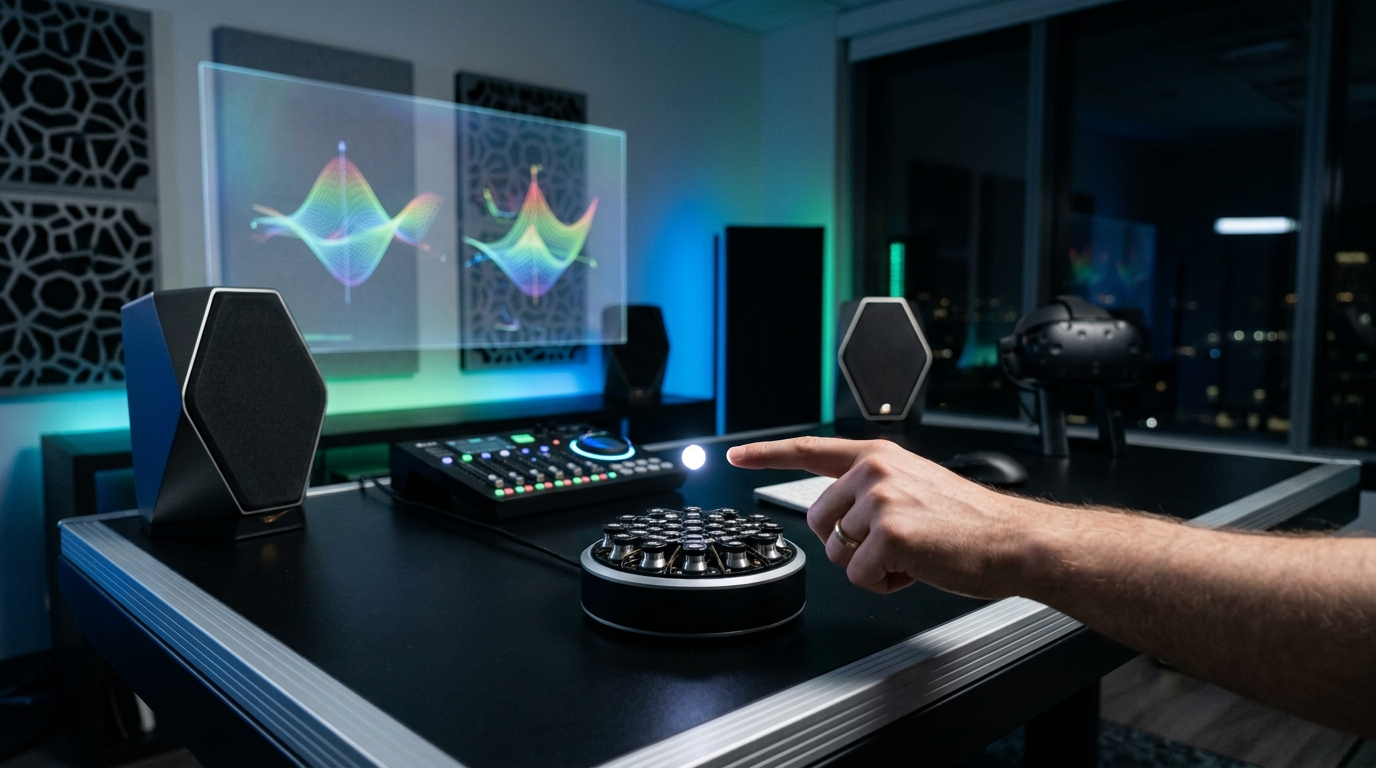
\includegraphics[width=\linewidth]{fig4.jpg}
    \caption{Interactive spatial audio application showing mid-air tactile particle manipulation and free-space visual anchor integration in an acoustic laboratory environment.}
    \label{fig:bose_ux}
\end{figure}

\subsection{Acoustic Field Visualization \& Transducer Calibration}
Serves as a physical embodiment of SEFI, rendering acoustic energy distributions, wave interference patterns, curvature, and multi-layered field structures in mid-air[cite: 2]. It provides an experimental benchmark for testing phase manipulation, standing wave node stability, transducer phase control, and non-linear acoustic radiation forces[cite: 2].

\subsection{Mixed Reality and Spatial Audio Interaction}
Acts as a physical free-space cursor or spatial sound anchor, combining physical visual cues with directional audio transducers for spatial audio UX paradigms[cite: 2].

\section{Conclusion}
This paper presents a volumetric rendering system that uses acoustic levitation to position and manipulate a single illuminated particle as a dynamic voxel[cite: 2]. By integrating established ultrasonic control techniques with a geometric field model, the system produces expressive three-dimensional structures through persistence of vision[cite: 2]. The Single Entity Field Interpretation (SEFI) provides the mathematical foundation for generating worldlines, curvature fields, and layered constructs, which are translated directly into real-time voxel trajectories[cite: 2].

The system's architecture is compact, low-cost, and grounded in well-validated physical principles[cite: 2]. Its modular control pipeline enables stable and precise voxel motion, and the resulting volumetric traces offer a clear method for visualizing geometric and acoustic phenomena[cite: 2]. By demonstrating that complex geometric structures can be rendered using a single levitated voxel, the system establishes a foundation for future volumetric display and spatial acoustic technologies[cite: 2].

\end{document}
